We present a unified infrastructure to support Deep FAIR for relational mathematical data.
It builds on our MathHub system, a portal for narrative and symbolic mathematical data.
\dmh is a part of the MathHub portal and provides storage and hosting with integrated support for Deep FAIR.
In the future, this will also allow for the development of mathematical query languages (i.e., queries that abstract from the encoding) and mathematical validation (e.g., type-checking relative to the mathematical types, not the database types).

\paragraph{Census of relational data in mathematics}
In some areas of mathematics, research products can consist of
listings or tabulations of complex mathematical objects and their properties.
These datasets can later be used by researchers to form or refute conjectures.
To facilitate the collection of information about relational data in mathematics,
we set up a database with a website frontend~\cite{bercic:cmo:table}.
The ``relational data'' part of Figure~\ref{fig:datasets} is a subset of this database.
While it grew out of the necessity to keep track of the information, 
it has at least two further goals.
First, it aims to make it easy for anyone to see what information has been collected so far.
Second, it aims to eventually make it easy to contribute information.

\begin{figure}[ht]
  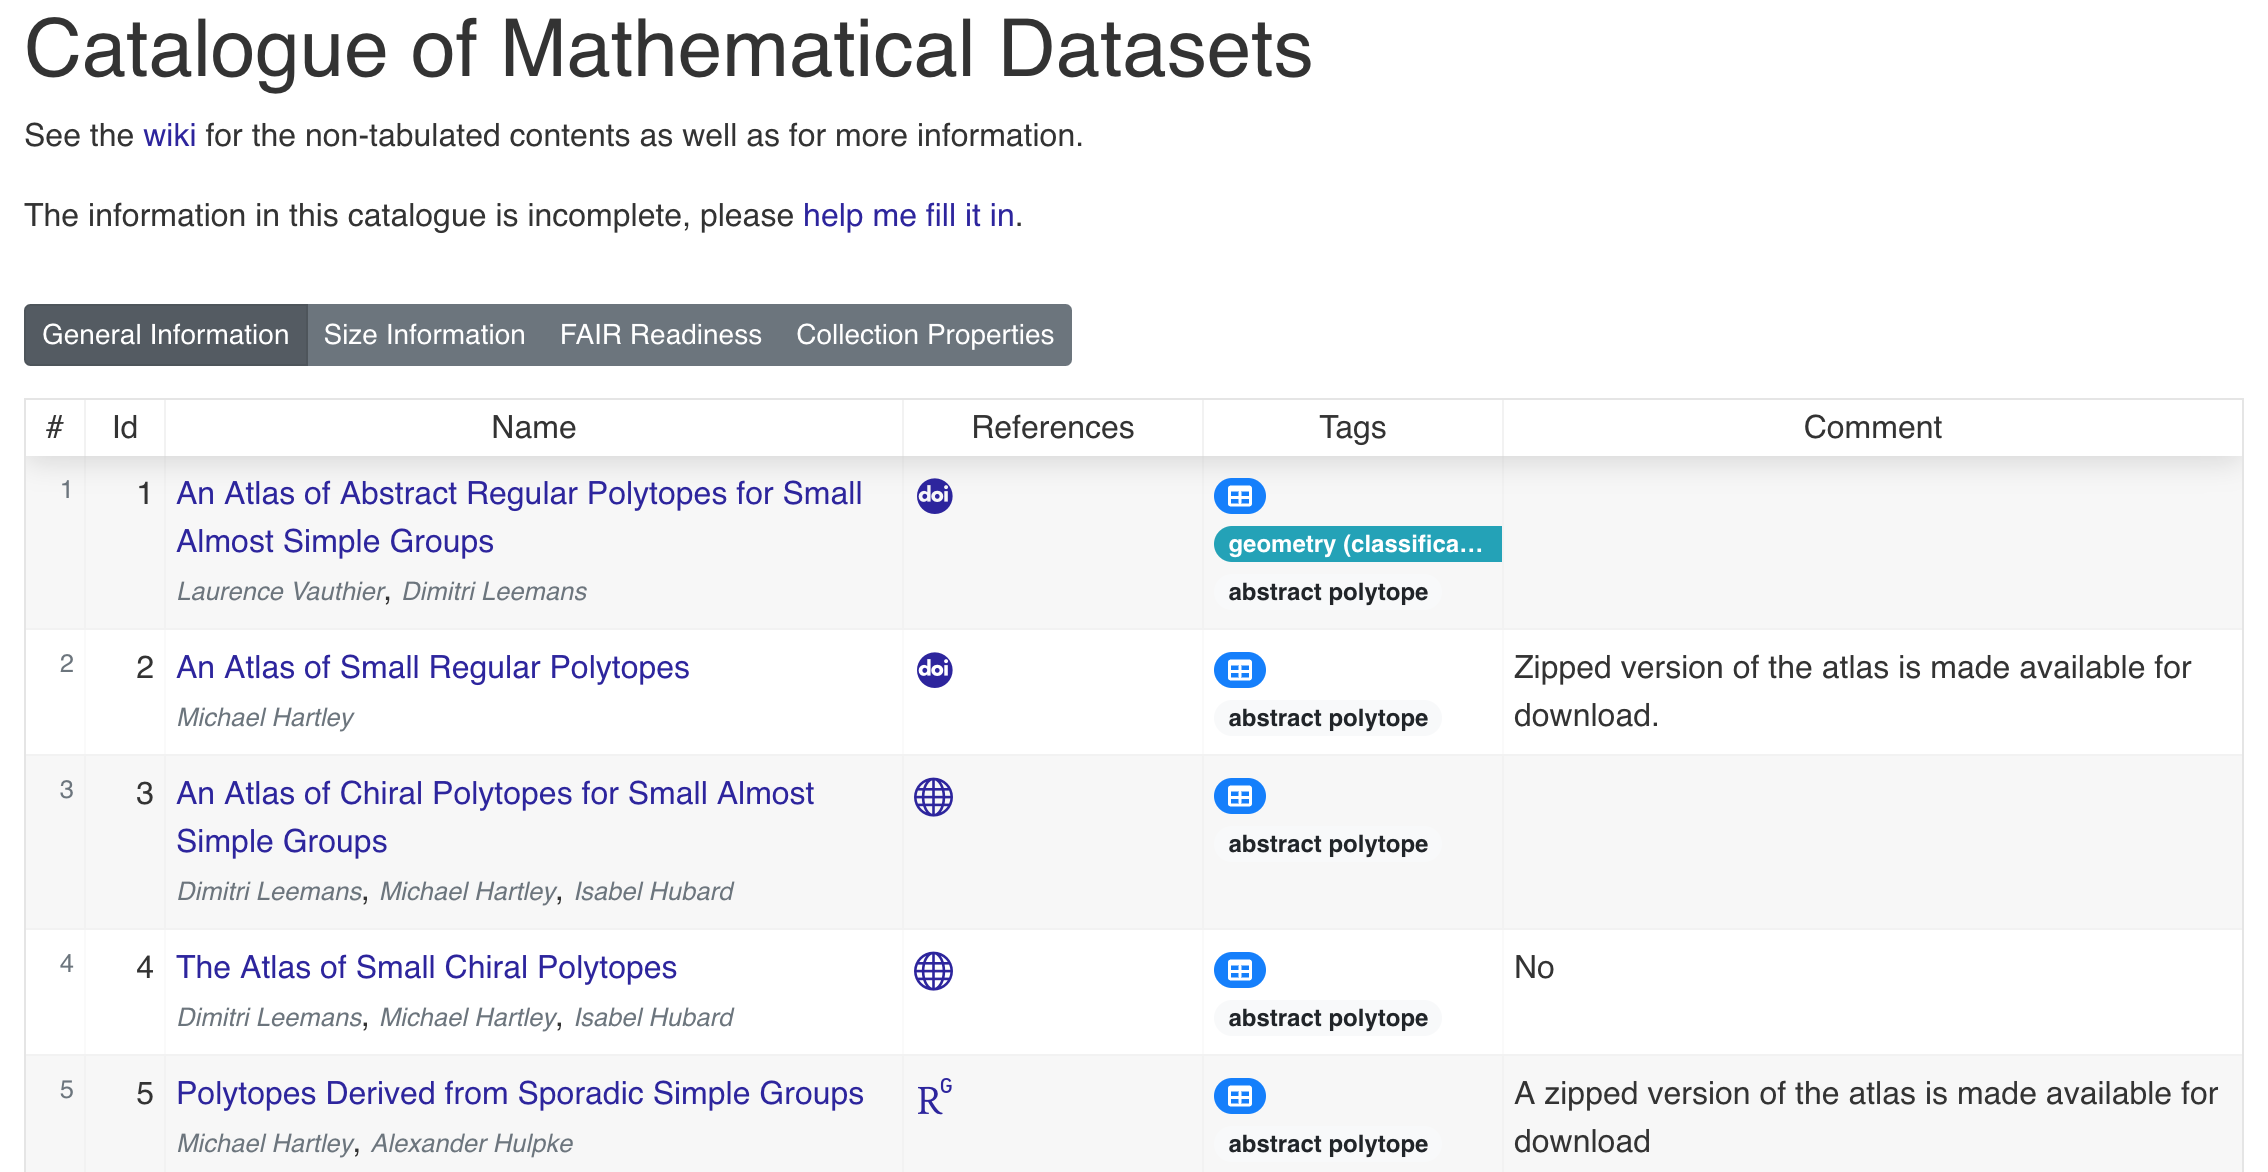
\includegraphics[width=\textwidth]{mathdb}
  \caption{Census website}\label{fig:census}
\end{figure}

The information about the datasets can be displayed in different views
(with switching implemented through tabs): 
general information, information about size, 
information pertaining to the FAIR principles,
as well as some other properties.

Currently, the census contains about $70$ datasets from several areas of mathematics.
This includes links to dataset websites and author information for (nearly) all of the datasets,
as well as literature references, area of mathematics and size-related information for many.
Even this small sample shows large variations in terms of
structure, content organisation, provenance, infrastructure and shareability, and size.

Perhaps the most important immediate use for this census is as a 
``market study'' for \dmh.
It serves as a source of use cases for the infrastructure,
as well as beginnings of a community of researchers that work with mathematical data.
Even in this initial stage, the census gives the developers of \dmh
some idea of the requirements for the system in terms of the ranges of
dataset size, complexity, etc.

We will continue to gather information about the relational datasets 
in mathematics in the living census website.
Finally, we plan to use the new information as a basis for a more structured census.

\paragraph{Mathematical data description language (MDDL)}
We developed a mathematical data description language MDDL in~\cite{BerKohRab:tumdi19} (Math Data Description Language) that uses symbolic data to specify the semantics of relational data.
MDDL schemas combine the low-level schemas of relational database with high-level specifications
(which critically use symbolic mathematical data) of the mathematical types of the data in the tables.

\begin{figure}[ht]
  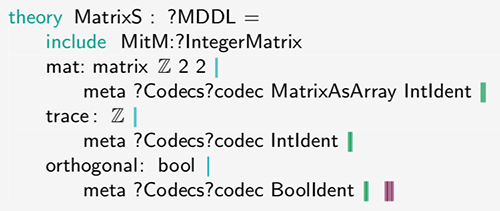
\includegraphics[width=.48\textwidth]{data_joe-schema}
  \caption{Schema theory for Joe's dataset}\label{fig:joe-schema}
\end{figure}

To fortify our intuition let us assume that Joe has collected a set of integer matrices together with their trace
and the Boolean property whether they are orthogonal.
Figure~\ref{fig:joe-schema} shows a MDDL theory that describes his database schema.
For example, the mathematical type of the field $\mathsf{mat}$ is integer $2\times2$ matrices;
the $\mathsf{codec}$ annotation specifies how this mathematical type is be encoded as a low-level database type (in this case: arrays of integers).
Concretely, the codec is the $\mathsf{MatrixAsArray}$ codec operator applied to the identity codec \footnote{
  Here `identity codec' means that mathematical integers are stored straightforwardly as database integers.
  This is not an identity in the mathematical sense, as e.g. integers larger than $64$ bit can not be stored in the database like this.
} for integers.
These codec annotations capture the representation theorem that allows representing the mathematical objects as ground data that can be stored in databases. 
%The tag \textsf{opaque} specifies that matrices cannot be used for filtering in the user interface. 

The information is sufficient to generate the datasets-specific components,
including a web interface.
The generation of APIs for computational software such as computer algebra systems 
is also possible and currently under development.
We describe this in more detail in the following section.

\paragraph{Description of the \dmh prototype}
The prototype uses MDDL dataset descriptions to produce the necessary infrastructure for each dataset.
The concept of codecs is crucial in the sense that they transparently connect 
the mathematical level of specification with the database level -- 
a critical prerequisite for the deep FAIR properties postulated above.
Moreover, in Figure~\ref{fig:joe-schema}, the mathematical background knowledge is 
imported from a theory $\mathsf{IntegerMatrix}$ in the Math In The Middle ontology (MitM)~\cite{MitM:on}, 
which supplies the full mathematical specification and thus the basis for \emph{Interoperability} and \emph{Reusability}; see~\cite{BerKohRab:tumdi19,WieKohRab:vtuimkb17,KohMuePfe:kbimss17} for details.
The overhead of having to specify the semantics of the mathematical data is offset by the fact that we can reuse central resources like the MitM ontology and codec collection. 
Thus, MitM and MDDL form the nucleus of a common vocabulary for typical mathematical relational datasets. 
%These can and should eventually be linked to representation standards in other domains. 
%For mathematical datasets, the math-specific aspects attacked by our work are the dominant factor.

\begin{figure}[ht]
  \includegraphics[width=0.8\textwidth]{DMH_infra.pdf}
  \caption{\dmh Infrastructure}\label{fig:dmhstruct}
\end{figure}

Currently, the infrastructure produced includes everything necessary to display a simple website with basic search functionality. 
The interface is shown in Figure~\ref{fig:joe}, its structure in Figure~\ref{fig:dmhstruct}.
The infrastructure consists of four main parts - a database (currently either Postgres of Sqlite), a backend (written in Django), a frontend (running inside the users' browser and written in React), and a data importer.

To import data into system we start with an MDDL description of the dataset. 
This is used to generate a so-called schema. 
The schema takes the form of a JSON file and aggregates all information required for the system as a whole to function. 
This schema contains all dataset properties along with the codecs used for them, all human-readable dataset descriptions and other meta-data. 
In a first step, the importer records all this information inside the database. 

Next, the encoded data is provided to the importer in the form of one or several JSON files. 
The importer can then use this file, and the schema, to interpret each value correctly and store it inside the database, concluding the import. 
During this process the importer also records appropriate data provenance. 

The frontend of the system is written in the React web framework.
It runs inside the users' browser and communicates with the backend via REST. 
Currently, it enables two main tasks: displaying all data inside a specific dataset, 
and searching for data subject to specific criteria. 

The frontend first requests the list of properties and used codecs from the backend. 
Based on this information, it then uses the appropriate UI components to build a search interface or present the specific values. 
This architecture implies that apart from adding support for new codecs, neither the frontend nor the backend code needs to be changed when a new dataset becomes available. 

\begin{figure}[ht]
  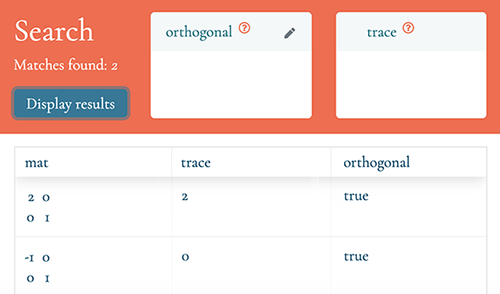
\includegraphics{data_joe.png}
  \caption{Website for Joe's dataset}\label{fig:joe}
\end{figure}

\medskip

\emph{The \dmh Data Model.}
The data model can be seen in Figure~\ref{fig:data-model}.
The following concepts appear in the data model.
\begin{itemize}
\item A \textbf{datum} is the atomic concept in the system.
Every datum belongs to a dataset.
It gives a value for some property of some item.
It has a provenance and is represented with a codec.
We can not eliminate the possibility of encountering more than one value
for a property of an item---this could happen due to a computational error.

\item A \textbf{dataset} corresponds to a single research product
and consists of a set of single data items (\emph{datum}s).
It combines information about the items it contains,
the properties (mathematical invariants) each item has,
which codecs are used to encode the actual values,
and finally, the provenances of all data contained in it.
The datasets can overlap non-trivially, e.g. the smaller graphs in the Census of Cubic Vertex-Transitive Graphs\footnote{http://staff.matapp.unimib.it/~spiga/census.html}
also appear in the list of Transitive Graphs\footnote{http://staffhome.ecm.uwa.edu.au/~00013890/remote/trans/index.html},
which also contains graphs of other degrees.

\item An \textbf{item} is a single mathematical object, 
represented in the system simply by a unique identifier.
Examples of these include groups, graphs, lattices, and other complex mathematical objects.
An item can belong to more than one dataset:
the Petersen graph naturally appears in both previously mentioned censuses.

\item \textbf{Provenance} is information on how and under which conditions each datum was produced.
Note that a datum can have more than one provenance.
This happens whenever the value of a property of an item is
computed independently in different datasets.

\item A \textbf{property} is a mathematical invariant of a mathematical structure.
An example of such a property is orthogonality of a matrix.
A property can be encoded in several ways
(recall the case of integers in LMFDB, where three different encodings are used).
Encodings of objects (such as the \texttt{graph6} representation for graphs)
are a special case of properties.

\item A \textbf{codec} is a pair of partial mappings between 
mathematical values of properties and the values represented in the database.
A codec combines the concepts of
\begin{itemize}
\item a \emph{mathematical type},
\item \emph{condition operators}, and
\item a \emph{database type}
\end{itemize}
with interface components such as a presenter (value display, possibly via a view) and condition widgets.
We will describe codecs in more detail in the following section.
\end{itemize}

\begin{figure}[ht]
  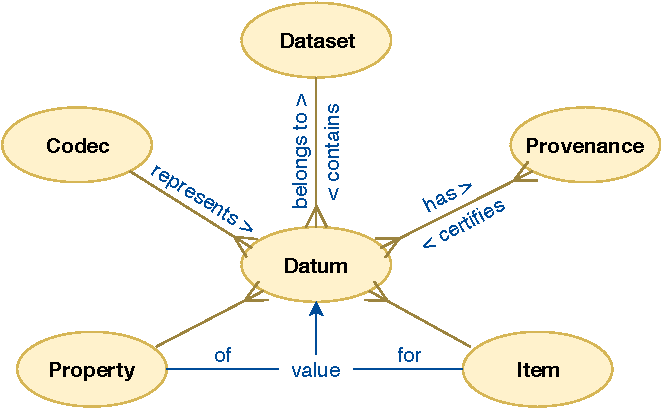
\includegraphics[width=0.6\textwidth]{data-model.pdf}
  \caption{Diagram of the \dmh data model}\label{fig:data-model}
\end{figure}

This data model already works well over the large set of examples we have examined so far.
To support more datasets, we will add further concepts in the future.
One of the concepts we want to add are ``Aggregated Datasets''. 
These are composed of several datasets and will introduce support for databases such as the OEIS\cite{Sloane:OEIS} or House of Graphs\cite{HOG:journal}.
These curated datasets are composed of a large number of smaller contributions.

\medskip

\emph{Codecs} are the glue that bind the data to the semantics and the MitM ontology.
They also separate the mathematical meaning from the implementation.
This separation of concerns enables optimising the mathematical layer (including the interface)
and the database implementation separately.
These two layers have fundamentally different goals: 
mathematicians (the users) do not care about the representation of data.
On the other hand, the implementation needs 
different representations of the data for different purposes.
For \dmh we expanded the notion of codecs as used previously in \pn~\cite{WieKohRab:vtuimkb17}
to include information for the interface.
\begin{figure}[ht]
  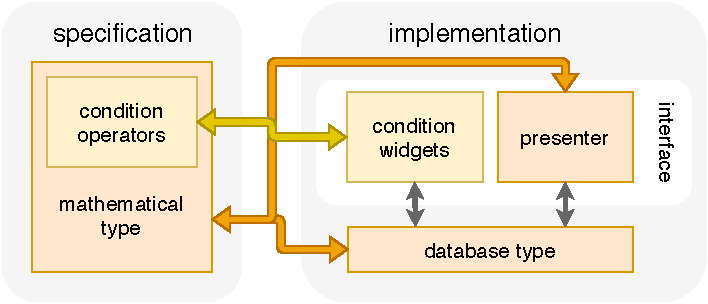
\includegraphics{codec.pdf}
  \caption{Diagram of information held by a \dmh codec}\label{fig:codec}
\end{figure}


For example, let us consider one of the basic codecs, \texttt{StandardInt}.
This codec encodes elements of $\mathbb{Z}$ (mathematical type) 
as standard $64$-bit integers (the database type).
The current list of condition operators given a constant $c$ contains the following unary operators:
$$
\begin{array}{ccc}
x \rightarrow x < c \qquad & \qquad x \rightarrow x > c \qquad & \qquad x \rightarrow x = c \\
x \rightarrow x \leq c \qquad & \qquad x \rightarrow x \geq c \qquad & \qquad x \rightarrow x \neq c
\end{array}
$$
The condition widget in the interface allows the user to enter the operator as a string,
for example \texttt{"<3"}.
This then gets mapped to a corresponding query at the database level.
Finally, the presenter is direct and simply displays the integer value.


\paragraph{The Workshop on Mathematical Data.}
 in Cernay, France (August 17-24th),
was dedicated to improving the status of relational data in mathematics.
The workshop brought together interested users and authors of mathematical datasets, 
data framework developers, 
and experts interested in integrating mathematical databases with computer algebra systems.
The workshop enabled progress on several fronts,
including major steps in the development of \dmh.
These included improving the architecture and model, 
as well as importing several real-life datasets into the system.
We sketched out a submission and editorial process for the platform.
We discussed provenance of data in mathematics and
drafted a standard and formalisation of math data provenance.

At the workshop, Dr. Andrea Kohlhase tested the user experience
of the existing web interface through user interviews.
The following points summarise the results of the user interface analysis.
\begin{itemize}
\item Users want easy access to definitions of concepts.
\item Users would appreciate having an interface in their language.
\item The search area and the result set area need to be consistent, or clearly indicate when they are not.
\item Users want to edit the view of the result set.
They want to select the columns they want to see as well as be able to reorder them.
In particular, they may or may not want to see the columns corresponding to the conditions they chose.
\item Users need to sort the result set, possibly by more than one column.
\item Good defaults need to be set for which columns are visible initially and how they are ordered.
\item Users want to export a whole dataset or a result set to Gap, Sage, Excel/CVS, etc.
\item Users need to be able to combine simple conditions on properties into more complex filters.
Composing the atomic conditions with logical \texttt{OR}, negation, \texttt{IF} in addition to \texttt{AND} would be welcome.
\item A user needs to be able to share the link to their search.
\end{itemize}
A detailed list of issues identified through the interviews is available at the 
workshop repository\footnote{https://github.com/OpenDreamKit/MathDataWorkshop/issues/3}.
Dr. Andrea Kohlhase also produced a clickable prototype of an updated interface
and used that in a few interviews combined with an eye-tracker test.

\paragraph{Conclusions and Evaluation}
Discussions on the user interface showed that the system will need to support contributors beyond dataset authors and infrastructure developers.
The interface
\begin{itemize}
\item would reach more users if it were available in multiple languages,
\item needs to show definitions of concepts,
\item needs to have good defaults for ordering of conditions and columns, and
\item needs to have good defaults for which columns are visible.
\end{itemize}
All of these features are valuable, since they make the system more usable.
However, it can not fall to the infrastructure developers or the dataset authors to provide the information necessary to support them:
On one hand, they require domain specific knowledge the infrastructure developers can not be expected to have.
They also represent a significant amount of effort and should not be done by the authors themselves.

Incidentally, the workshop showed that it can be fruitful to bring together  researchers who know what kind of datasets their community would benefit from and researchers who know how to generate such datasets.
One such collaboration started at the workshop.

\emph{Finally, but probably most importantly, 
the workshop showed that the research community accepts the idea of a system like \dmh
and is taking it seriously to the extent that several participants offered help with tasks such as dataset reviews.}
%\end{mdframed}

%%% Local Variables:
%%% mode: latex
%%% mode: visual-line
%%% fill-column: 5000
%%% TeX-master: "report"
%%% End:

%  LocalWords:  flexiformal BerKohRab:tumdi19 includegraphics textwidth textbf textsf textsf textsf ednote BerKohRab:tumdi19,WieKohRab:vtuimkb17,KohMuePfe:kbimss17 externalize Cernay shareability mathsf emph emph dmh fig:dmhstruct medskip mathbb rightarrow qquad qquad rightarrow qquad qquad rightarrow leq geq neq mathdb WieKohRab:vtuimkb17
